%%%%%%%%%%%%%%%%%%%%%%%%%%%%%%%%%%%%%%%%%%%%%%%%%%%%%%%%%%%%%%
\section{Composing \Xxing Transformations}
\label{s:composition}

\begin{comment}
\begin{figure}[h]
    \centering
    \small
    \begin{tabular}{c|c|c|c} %|m{0.08\linewidth}}
        Operation & Remove & Modify & Decorrelate \\
        \hline
        Remove & $\varnothing$ & $\varnothing$ & $\varnothing$\\ 
        \hline
        Modify & Remove data & Modify data & Decorrelate data\\ 
        \hline
        Decorrelate & Remove data$^*$ & Modify data$^*$ & Recursively decorrelate data$^*$\\ 
    \end{tabular}
    \caption{What happens when disguise operations compose, with the first
    operation on the vertical, and the second operation on the horizontal. $^*$
    represents operations that require special handling, using the user's reveal
    credentials to find previously-decorrelated data to disguise and recursively
    disguise them.}
    \label{tab:composition}
\end{figure}
\end{comment}

\sys supports composition of \xxing transformations, which occurs when a
transformation applies to data that \sys has previously \xxed in
some other way.
%
Reasoning about composition of transformations can be broken into reasoning
about the composition of primitive operation pairs, \eg remove after
modify, or remove after decorrelation.
%

%
Many pairs result in trivial composition: no operation can be composed after a
remove (the data is gone), and any operation after a modify updates the
data as expected. 
%
However, operations after decorrelation result in more complex composition scenarios.
%
For instance, decorrelation after decorrelation could occur if a user
decorrelates some posts, after which an administrator decorrelates \emph{all}
posts (\eg to anonymize all inactive users). In this scenario, the administrator's \xxing operation applies to
pseudoprincipal-owned posts in the same way as it does to unmodified posts. This
creates pseudoprincipals that can speak-for other pseudoprincipals.  This notion
of chaining together pseudoprincipals creates \sys's \emph{speaks-for chains}.
\sys uses the pseudoprincipal's registered public key to encrypt pseudoprincipal
diff and speaks-for records, so \sys does not need to know its link to an
original principal in order to encrypt and \xx its data.
%

%
%For instance, a user could decorrelate their posts, after which an
%administrator could modify all posts (including those of pseudoprincipals) by
%removing associated metadata.
%

%Another interesting case is when a transformation should apply to data that a
%user owned, but that has already been decorrelated.
Removal or modification after decorrelation also require special handling. For
instance, a Lobsters user might first decorrelate some of their comments and
then request to delete all their comments (\eg by deleting their account).
%
But the decorrelated comments are no
longer linked to the original user; how can the deletion transformation find
them?
%
\begin{comment}
%\sys by default handles \xxing of previously modified or decorrelated data
%without any problems: pseudoprincipals have affiliated public keys, and \sys
%treats them the same as any other principal when \eg an administrator wants to
%\xx all users' posts.
%
%Users can reveal \xxed data on behalf of their pseudoprincipals as described in
%\S\ref{s:reveal}.
\end{comment}
%
\sys addresses this question by accepting optional reveal credentials as part of
the \xx operation (the \texttt{disguise\_over} argument of \sys's
\texttt{DisguiseData} API call).
%
Reveal credentials let \sys recursively decrypt speaks-for records and create a
speaks-for chain starting from the disguising user, represented by speaks-for
relationships between pseudoprincipals. \sys can then disguise all data of all
pseudoprincipals included in the speaks-for chain.
%

With reveal credentials, \sys decrypts the user's previous diff and speaks-for
records. Each speaks-for record includes the identifier for one of the user's
pseudoprincipal and the pseudoprincipal's private key, and creates a ``link'' in
the speaks-for chain. A pseudoprincipal's identifier allows \sys to find data
referencing that pseudoprincipal and apply \xxing transformations on behalf of
the this pseudoprincipal as well as the user. 
%
A pseudoprincipal's private key---its reveal credentials---allows \sys to
recursively decrypt its speaks-for records, and disguise any pseudoprincipals of
this pseudoprincipal created by multiple decorrelations.
%

%When decrypting a 
%\sys uses pseudoprincipal private keys in decrypted speaks-for records as
%credentials to recursively find pseudoprincipals from multiple decorrelations.

%
%\begin{comment}
%This lets \sys support Lobsters users first decorrelating their data, and then
%removing (or modifying) it via an additional \xxing transformations applied
%with their reveal credentials.
%\end{comment}
%\lyt{Without reveal credentials, \sys would not \xx any of the
%user's data previously decorrelated to pseudoprincipals.}
%and include them in the query to the application database.
%

\paragraph{Out-of-Order Reveals.}
\label{s:design:oooreveals}

\begin{figure}
\centering
    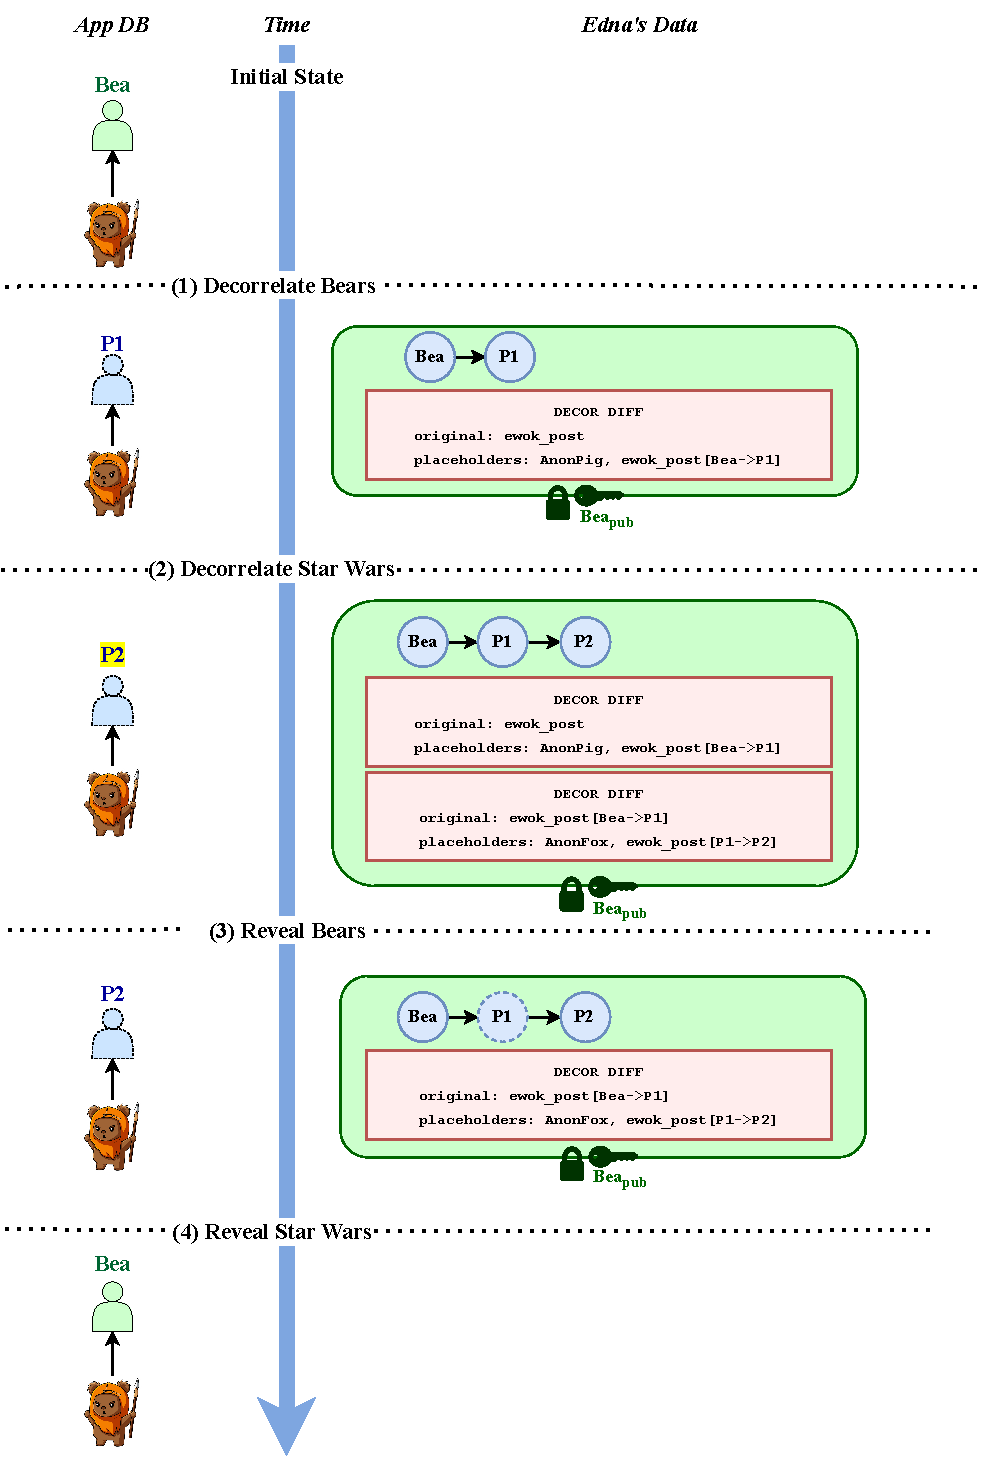
\includegraphics[width=0.82\textwidth]{figs/composition}
    \caption[Decorrelations can compose and be revealed in any order.]
    {\small \sys allows multiple decorrelations to compose, and can reveal them in
    any order such that the data remains decorrelated until the user reveals \emph{all}
    applied decorrelations. The speaks-for chain encoded in
    speaks-for records (shown in blue) allows \sys to handle recorrelation of intermediate
    pseudoprincipals. When Bea requests reveal of their ``Star Wars''
    posts (4) after revealing ``bears'' posts (3), \sys walks the speaks-for chain
    backwards from $P_2$ to find the latest principal that can speak-for $P_2$
    and has not yet been recorrelated. Thus, \sys restores ownership back to
    Bea.}
\label{f:composition-desn}
\end{figure}


\sys must also handle reveals of transformations in any order.  As before,
many scenarios are straightforward: revealing removals is trivial (data can
only be removed and restored once), and revealing modified data simply restores
the original (subject to consistency checks).
%
Handling out-of-order reveals of multiple decorrelations presents the greatest
challenge.
%
\sys's semantics (\S\ref{s:semantics:hl}) require that data that is decorrelated
multiple times will not be recorrelated until all \xxs are removed.
%also enables another desirable form of
%\xxing composition: .
%One desirable form of \xxing composition required special support:
%
For example, as shown in Figure~\ref{f:composition-desn} (left-hand side), if Bea
separately decorrelates their comments on ``bears'' and ``Star Wars'' posts,
then later reveals the ``bears'' posts, they might want Ewok-related comments
(tagged both ``Star Wars'' and ``bears'') to remain \xxed, even though they were
initially \xxed under the ``bears'' transformation.
%
%To realize this, \sys lets a \xxing transformation recursively operate over
%pseudoprincipals' data when their \emph{owner} (authorized through credentials
%that let them access a speaks-for record) invokes it.
%
%With reveal credentials, \sys finds pseudoprincipals with
%already-decorrelated comments and applies the \xxing transformation to these
%pseudoprincipals. This again creates pseudoprincipals that can speak-for other
%pseudoprincipals.
%
To support this, \sys again uses the speaks-for chain (\S\ref{s:composition}) to
find pseudoprincipals stemming from the revealing user.
%
All reveal operations walk the full speaks-for chain to reveal all necessary
records (cf.\ Figure~\ref{f:revealpseudo}).

Furthermore, if reveal operations perform recorrelations out of order, \sys
removes an intermediate link in the speaks-for chain.
%
To describe how this works, take the example of two disguises that decorrelate
comments on ``bears'' and ``Star Wars'' posts respectively
(Figure~\ref{f:composition-desn}). 

%
\begin{enumerate}
    \item[(1)] First, the ``bears'' decorrelation rewrites Ewok posts to
        pseudoprincipal $P_1$. Bea's disguised data includes a speaks-for record
        from Bea to $P_1$ and a diff record recording the database changes.
%
\item[(2)] Next, a ``Star Wars'' decorrelation composes on top of the ``bears''
    decorrelation to rewrite Ewok posts from $P_1$ to pseudoprincipal $P_2$.
        This creates disguised data for $P_1$, including a speaks-for record
        from $P_1$ to $P_2$ and a diff record recording the database changes.
%
        At this point, \sys has speaks-for records originating from Bea that encode
        a speaks-for chain from Bea $\to P_1 \to P_2$.
%
\item[(3)] If Bea first reveals the ``bears'' anonymization---the first applied
disguise---on their data, \sys finds all accessible speaks-for records given
Bea's reveal credentials (cf.\ Figure~\ref{f:revealpseudo}), and constructs Bea's
speaks-for chain as a graph of principal-to-principal edges (namely Bea$\to
P_1\to P_2$).
%
\sys finds that $P_1$'s ``Ewok'' posts no longer exist in the database (they
        belong to $P_2$ due to the composed ``Star Wars'' disguise), and thus
        does not restore ``Ewok'' posts to Bea. \sys does still remove
        pseudoprincipal $P_1$ in the process of restoring ``bear'' diff records,
        and once done, clears all ``bear'' diff records from its encrypted
        disguise table. 
%
        Importantly, however, \sys still retains the speaks-for record for
        Bea$\to P_1$, since $P_1$ still has associated disguised data (namely a
        speaks-for record to $P_2$ and a diff record).
%
\item[(4)] Now, if Bea reveals the second applied disguise---``Star
    Wars''---\sys sees that $P_1$'s diff record has an original row with $P_1$ as
        owner. 
%
        However, \sys cannot reveal the diff record directly and restore the
        decorrelated posts to $P_1$, as this will fail referential integrity
        consistency checks. Furthermore, the reveal of ``Star Wars'' reveals the
        last disguise applying to Bea's posts, so \sys should restore posts to
        their original, undisguised state (instead of decorrelated to $P_1$).

        Instead of immediately revealing the diff record, \sys walks the
        speaks-for chain (Bea$\to P_1 \to P_2$) backwards from $P_2$ to
        determine the \emph{next valid} principal in the chain who speaks-for $P_2$,
        which in this case is Bea.
        %
        A valid principal can either be a natural principal or a pseudoprincipal
        yet to be recorrelated. If a pseudoprincipal appears as placeholder data
        in any diff record of Bea's disguised data (from any disguise), \sys
        knows that it has not yet revealed that pseudoprincipal. Had \sys
        revealed that pseudoprincipal, then \sys would have removed its
        corresponding diff
        record.
        %

%
        After determining that Bea is the next valid user in the speaks-for chain to
        $P_2$, \sys rewrites the removed ``Ewok'' row in the diff record so that
        it references Bea instead of $P_1$, and then restores the rewritten row
        to the database. \sys also removes pseudoprincipal $P_2$.
%
        Finally, \sys deletes the diff record for the ``Star Wars'' disguise, as
        well as
        $P_2$ and $P_1$'s speaks-for records (since both pseudoprincipals 
        have no associated disguised data).
        This implicitly truncates the speaks-for chain to just Bea.
        %
\end{enumerate}
%
%This design works even in the presence of multiple recursive decorrelations and
%many-link speaks-for chains. 
\sys enforces the invariant that the chain stops at some principal $P$ only once all pseudoprincipals recursively generated in the chain beyond $P$ have
been recorrelated.
%

%%%%%%%%%%%%%%%%%%%%%%%%%%%%%%%%%%%%%%%%%%%%%%%%%%%%%%%%%%%%%%%%%%%%%%%%

%
%(in which case,
%an earlier link in the speaks-for chain may be removed).
%Pseudoprincipal-to-pseudoprincipal speaks-for relationships requires special
%handling during reveal operations: \sys %which must ensure that chains of speaks-for records remain linked to the
%original user even if reveal operations are applied out of order.

\begin{comment}

    To prevent such revealing behaviors, the user must provide their reveal
    credentials to tell \sys which pseudoprincipals the user can speak-for and
    whose data the user can recursively \xx.
%
    If Lobsters requires Bea to provide their reveal credentials when \xxing
    ``sci-fi'', \sys can then use those credentials to get Bea's speaks-for
    records, which relate Bea to any pseudoprincipal created for their ``Star
    Wars'' content.
%
    Equipped with the knowledge of these pseudoprincipals, \sys can now find
    comments that have the ``sci-fi'' tag \emph{even if} they also have the
    ``Star Wars'' tag (and thus have been already decorrelated).
%
    \sys then recursively decorrelates these dually-tagged comments from Bea's
    existing pseudoprincipals.
    %Rather than create a speaks-for record from \emph{Bea} to a new
    %pseudoprincipal , for these comments, \sys creates speaks-for records from
    %$p$ to $q$.
%

%
    Recursive decorrelation creates a chain of speaks-for records in \sys that
    ensures correct behavior on revealing.
%
    If Bea reveals their ``sci-fi'' comments first, the comments simply revert
    to being owned by Bea's pseudoprincipals.
%
    If Bea reveals their ``Star Wars'' comments first, \sys detects that
    dually-tagged comments are associated with another layer of pseudoprincipals
    in the application database, and does not reassociate them; instead, \sys
    simply
    %since the ``sci-fi'' \xxing transformation decorrelated the comment yet
    %again.
%
    %Comments with both tags continue to be owned by $q$, because \sys's reveal
    %process leaves modifications to the application database in place if they
    %happened after \sys applied the transformation it is currently revealing.
%
    internally updates the chain of speaks-for records so that only one layer of
    pseudoprincipals remain.

%
%
    %If Bea chooses to reveal the second transformation, \sys in both cases
    %reveals the original content, without having incorrectly revealed
    %``sci-fi'' comments in the intermediate state.
%
    %This composition is not a concern for votes, since the ``Star Wars''
    %\xxing transformation already removed them from application database.
%

%Lobsters expects that all ``sci-fi'' content decorrelated via category-based
%anonymization will remain decorrelated until Bea

\iffalse
% OUTLINE
% - introduce how pseudoprincipals are dealt with in the system
%    - have own keypair that is encrypted (chaining works)
%    - can own bags
%    - (encrypted) locators are kept as part of metadata for pseudoprincipald
% - process of chaining two \xxings
%       - go over steps in diagram (using example)
% - process of shared data
%       - use example of private messages here
An application may let a principal apply multiple \xxing transformations, some
of which may \xx data decorrelated to pseudoprincipals by some prior
transformation.
%
If data decorrelated by \xxing transformation $s$ could never be \xxed again,
then re-correlating the data by revealing $s$ might prematurely reveal data
\xxed by transformations applied after $s$.
%

\head{Composing Decorrelations.}
%
To solve this, \sys lets users \xx the data of pseudoprincipals that they can
speak-for.
%
This introduces a layer of indirection, so that revealing either transformation
will leave the decorrelating effects of the other in place.
%
To realize this indirection, \sys lets a \xxing transformation recursively
operate over pseudoprincipals' data when their \emph{owner} (authorized
through credentials that let them access a speaks-for record) invokes it.
%

%
In the example, \sys has access to Bea's reveal credentials when applying the
second \xxing transformation, so \sys can use those credentials to inspect any
of Bea's already-\xxed data.
%
This includes speaks-for records, which relate Bea to any pseudoprincipal $p$
created for their ``Star Wars'' content.
%
Equipped with the knowledge of these pseudoprincipals, \sys can now find
comments that have the ``sci-fi'' tag \emph{even if} they also have the ``Star
Wars'' tag (and thus have been already decorrelated).
%

%
Rather than create a speaks-for record from Bea to some new pseudoprincipal $q$
for these comments, \sys creates speaks-for records from $p$ to $q$.
%
This creates a chain of speaks-for records (Bea speaks-for $p$, which
speaks-for $q$) that ensures correct behavior on revealing.
%
If Bea reveals their ``sci-fi'' comments first, the comments simply revert to
being owned by $p$.
%
If Bea reveals their ``Star Wars'' comments first, \sys detects that these
comments are now owned by $q$ in the application database, since the ``sci-fi''
\xxing transformation changed the owner from $p$ to $q$.
%
Comments with both tags continue to be owned by $q$, because \sys's reveal
process leaves modifications to the application database in place if they
happened after \sys applied the transformation it is currently revealing.
%
\sys internally removes the mapping from Bea to $p$, and instead maps
Bea directly to $q$.
%
If Bea chooses to reveal the second transformation, \sys in both cases
reveals the original content, without having incorrectly revealed ``sci-fi''
comments in the intermediate state.
%

% --------------------------------------------------------------------------------

% Application of a new \xxing transformation $s_2$ on data \xxed
% by $s_1$ is relatively straightforward if $s_1$ only modified the data:
% %
% \sys encrypts stored records from $s_2$ with the associated principal’s public
% key, allowing that principal’s client to reveal the \xxing transformation by
% providing the corresponding private key. (\Xxing over data removed by $s_1$ is
% impossible because the data does not exist.)
% %
% However, if $s_1$ decorrelated data and reassociated it with pseudoprincipals,
% then $s_2$ cannot find the associated principal or its public key.
% %
% To solve this, \sys creates public/private keypairs for pseudoprincipals,
% encrypts pseudoprincipal data with pseudoprincipals' public keys, and lets a
% natural principal prove a speaks-for relationship with these pseudoprincipals.

% \lyt{Not sure if this is the right place...}
% In the following, we refer to all encrypted data that \sys produces when
% applying \xxing transformation $s$ as a \emph{bag}; locator \lcapa{ps} points
% to the bag of principal $p$'s \xxed data produced when applying $s$.

% %%%%%%%%%%%%%%%%%%%%%%%%%%%%%%%%%%%%%%%%%%%%%%%%%%%%%%%%%%
% \head{Storing Data for Pseudoprincipals.}
% %
% Each time \sys creates a new pseudoprincipal $q$ for natural principal $p$
% during $s_1$ (with $p$'s public key still available), it generates a keypair
% for $q$.
% %
% \sys then ``wraps'' $q$'s private key by encrypting it with $p$'s public key,
%  stores it with records created by $s_1$ at locator \lcapa{ps_1}, and
% forgets the plaintext private key.
% %stores it at bag pointed to by locator \lcapa{ps_1}, and
% %
% Hence, access to $q$'s private key---or records encrypted for $q$---requires $p$'s private key.
% %
% \sys then stores $q$'s public key via \fn{RegisterPrincipal} and uses it to encrypt $q$'s records.
% %
% This idea applies recursively: in the above example, $p$ itself may
% be a pseudoprincipal and not a natural principal.
% %
% (This is why the application cannot \eg simply email $q$'s private key to
% $p$ when it creates a pseudoprincipal $q$.)
% %
% In this case, \sys encrypts $q$'s private key with the public key of
% pseudoprincipal $p$, granting any natural principal who can access
% $p$'s private key access to $q$ and its data.
% %
% Thus, the bag at locator \lcapa{ps} contains both $p$'s encrypted records and
% pseudoprincipal private keys from \xxing transformation $s$.

% %%%%%%%%%%%%%%%%%%%%%%%%%%%%%%%%%%%%%%%%%%%%%%%%%%%%%%%%%%%
% \head{Pseudoprincipal Metadata.}
% %
% When $s_2$ creates a record bag encrypted for pseudoprincipal $q$, it produces
% locator \lcapa{qs_2} for the bag.
% %
% \sys stores this locator with pseudoprincipal $q$'s metadata, but encrypts
% it with $q$'s public key.
% %
% Encrypting pseudoprincipal locators ensures that \sys never exposes the mapping
% from a principal to its locators once a principal has \xxed their account (\sys
% returns all locators of natural principals to the application when \xxing, as
% described in \S\ref{s:design:\xxing}).
% %
% Locator \lcapa{qs_2} will only be needed to reveal $s_2$---and at that point,
% $q$'s private key will be available, as the principal who speaks-for $q$
% unwraps it.
% %

% %
% As an optimization, the application can tell \sys to return \lcapa{qs_2} instead
% of storing it; the application is then responsible to return the locator to
% the correct natural principal (\eg displaying a QR code to a client invoking $s_2$).
% %
% %$p$'s private key and bag locator \lcapa{ps_1} are available.
% %This causes \sys to return pseudoprincipal bag locators without
% This avoids an extra encryption per pseudoprincipal.
% %
% $p$ then reintroduces these locators when they reveal $s_2$.
% %

% \begin{figure}[t]
%     \centering
%     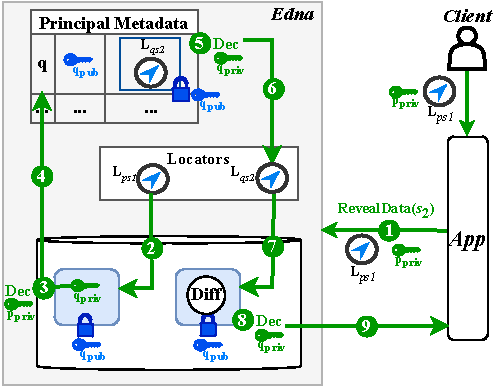
\includegraphics{figs/edna_reveal}
%     \caption{To retrieve diffs from composed \xxing transformation $s_2$, \sys
%              first decrypts $q$'s private key in $p$'s bag for $s_1$,
%              and uses that private key to decrypt \lcapa{qs_2} and the bag
%              it points to.}
%     \label{f:recursive}
% \end{figure}

% \newcommand*\circled[1]{\tikz[baseline=(char.base)]{
%             \node[shape=circle,draw,inner sep=1pt] (char) {#1};}}
% %
% Figure~\ref{f:recursive} shows how a natural principal reveals a composed
% \xxing transformation. %using the low-level API.
% %
% \lyt{(Added the following:)} In this example, clients provide private keys as reveal credentials.
% %
% \circled{1} The application asks \sys to reveal $s_2$ using $p$'s
% private key and \lcapa{ps_1}.
% %
% \circled{2}
% \sys looks up \lcapa{ps_1} to find $p$'s bag for $s_1$, and \circled{3}
% decrypts it with $p$'s private key.
% %
% This reveals that $s_1$ created pseudoprincipal $q$ and reveals $q$'s private
% key, so \circled{4} \sys looks up $q$'s metadata and
% \circled{5} decrypts $q$'s locators with $q$'s private key.
% %
% \circled{6} This provides \sys with \lcapa{qs_2}, so it \circled{7} looks
% up $q$'s bag for $s_2$, \circled{8} decrypts it with $q$'s private key,
% and finds the database diff applied for $q$ during $s_2$.
% %
% \circled{9} Finally, \sys reveals the \xxed data held in the diff,
% and returns to the application.
% %returns the diff to the application, which reveals the \xxing transformation.

% \head{Data Cleanup.}
% %
% When \sys reveals $s_1$ and recorrelates $p$ to its data, \sys removes both $q$
% and $q$'s public key from $q$'s metadata.
% %
% However, \sys must sometimes retain part of $q$'s metadata, as it may include
% encrypted locators that \sys must keep to later find $q$'s bags.
% %
% Given that \sys cannot decrypt $q$'s locators, nor send them to a client, \sys will still retain
% $q$'s metadata if the metadata contains encrypted locators after revealing.
% %when the application calls \fn{ForgetPrincipal} on $q$.
% %
% However, \sys marks $q$ as forgotten, so that \sys knows to delete $q$'s metadata when \sys clears
% all stored records at $q$'s locators during future \xxing transformation reveals.
% %

% %
% Because \sys may need to use \lcapa{ps_1} to access $q$'s encrypted private key, \sys retains $q$'s
% encrypted private key at \lcapa{ps_1} even if the rest of $s_1$'s \xxed data at
% \lcapa{ps_1} (\ie encrypted diff or speaks-for records) has been removed.
% %
% The bag is now empty except for $q$'s private key.
% %
% \lyt{Move to discussion?
% \sout{To hide that \sys deleted previously-stored data, it puts a random-length
% dummy record into the bag.}}
% %
% %Once \sys has removed $q$'s metadata, then \sys removes all trace of \lcapa{pd} since the
% %referenced bag is empty.
% %

% %
% %Natural principal $p$ fully reveals \xxing transformation $s_2$ by providing \lcapa{ps_1}: this locator must be
% %from the \xxing transformation $s_1$ that decorrelated $q$ from natural principal $p$.
% %
% To reveal $s_2$, \sys follows Figure~\ref{f:recursive} to find and reveal the
% records for $s_2$ at \lcapa{qs_2}. \sys also clears all records at \lcapa{qs_2}
% after revealing. Because $q$ has been marked forgotten, \sys then removes
% \lcapa{qs_2}, which points to a now-empty bag.
% %
% Once \sys has removed all metadata for $q$, \sys removes $q$'s private key and
% \lcapa{ps_1} since the bag is now empty.
%
\end{comment}
